% !TEX root=/home/tavant/these/manuscript/src/manuscript.tex

\section{Solving the kinetic \acs{DR} for general distribution functions}
  \label{sec-DR-solver}
  % \renewcommand\rightmark{\expandafter\MakeUppercase{Solver for the general DR}}


  In order to solve the \ac{DR}  $\hat\epsilon(\vect{k}, \omega) = 0$ of \cref{eq-drECDI}, we solve for every $\vect{k}$ the complex value of $\omega$ that is a zero, also named a root, of $\hat\epsilon(\vect{k}, \omega)$.
  Hence, we first need to evaluate $\hat\epsilon(\vect{k}, \omega)$ for any given arguments $\vect{k}, \omega$.
  Then, we can find the root.
  

  \subsection{Numerical determination of \texorpdfstring{$\hat\epsilon$}{the plasma dielectric function.}} \label{subsec-numepsilon}
  
  The calculation of $Z$, needed to determine $\hat{\epsilon}$, is usually done using the Maxwellian hypothesis \citep{cavalier2013} (hence using the Fried and Compte function $Z_M$), the kappa distribution \citep{ziebell2017}, or other analytic expressions.
  We can also use a linear combination of such simple distribution functions, such as done in the software WHAMP in \citet{ronnmark1982}.
  Here we propose to solve the dispersion relation $\hat{\epsilon}=0$ using the distribution function measured in the \ac{PIC} simulation.
  
  The numerical computation of $\norm{\hat\epsilon}$ is done using the method of \citet{xie2013} for computing $\tilde{Z}$ the numerical approximation of $Z$. 
  It uses the fact that $Z$ is an Hilbert transform of the distribution function, and that the Hilbert transform can be changed to a Fourier Transform, weighted by well chosen basis functions, so the \ac{FFT} algorithm can be used \citep{weideman1995}.
  An interesting point is that the evaluation of $\tilde{Z}(\eta)$ is done by a polynomial function, which coefficients depend only on the distribution function $f$. 
  Hence, they need to be determined only once, and evaluating $\tilde{Z}(\eta)$ is relatively fast.
  
  \begin{figure}[!hbt]
    \centering
    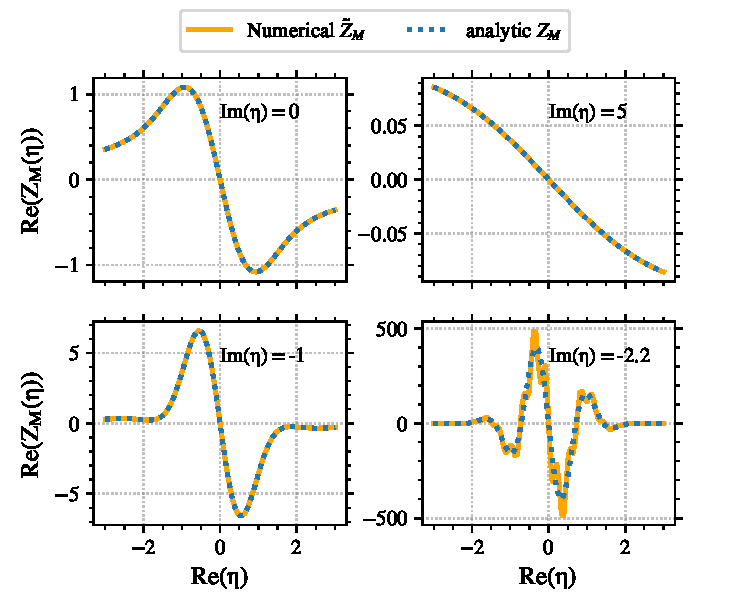
\includegraphics[width=0.8\textwidth]{Validation_numericalZ.pdf}
    \caption{Comparison of the numerical evaluation of $\tilde{Z}_M(\eta)$ for a Maxwellian distribution function with the Fried and Conte function (from the \texttt{plasmapy} python package) for different values of the imaginary part of $\eta: 5, 0,-1,$ and $-2.2$.  }
    \label{fig-numZ}
  \end{figure}
  \cref{fig-numZ} shows the comparison of the numerical evaluation of $\tilde{Z}(\eta)$ for a Maxwellian distribution function with the Fried and Conte function (from the \texttt{plasmapy} python package) for different values of the imaginary part of $\eta$.
  We can see that for ${\rm Im}(\eta)$ positive, null or slightly negative, the two functions gives exactly the same results.
  However, for larger negative values of ${\rm Im}(\eta)$, the two functions gives different results.
  
  This discrepancy between $Z_M$ and $\tilde{Z}_M$ for large negative imaginary argument is certainly due to the fact that the analytic expansion of $Z$ to the complex plane require the evaluation of the distribution function for complex velocities \citep{xie2013,weideman1995}.
  However, the discrete velocity distribution function measured in the \ac{PIC} simulation cannot be properly evaluated for complex velocities.
  On the other hand, we are only interested in instabilities, with positive growth rate.
  Hence, the discrepancy observed should not affect the conclusions of the study.
  


  \begin{figure}[hbt]
    \centering
    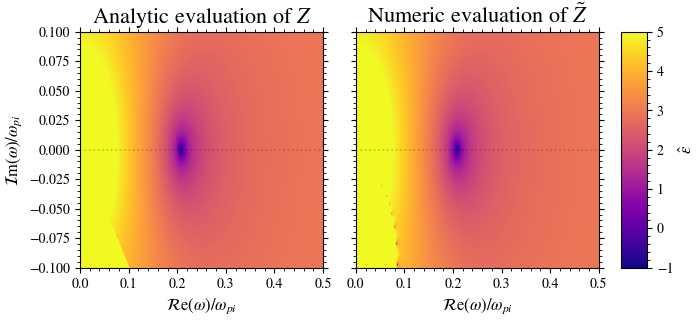
\includegraphics[width=0.8\textwidth]{Validation_numericalZ_bis.png}
    \caption{Comparison of the numerical evaluation of $\hat\epsilon$ from \cref{eq-drECDI} for a Maxwellian distribution function with (left) the Fried and Conte function (from the \texttt{plasmapy} python package) and (right) the numerical $\tilde{Z}$, in logarithmic scale.  }
    \label{fig-numZbis}
  \end{figure}
  
  \Cref{fig-numZbis} presents the comparison of the calculation of $\hat\epsilon$ from \cref{eq-drECDI} for a Maxwellian distribution function with (left) the Fried and Conte function (from the `plasmapy` python package) and (right) the numerical $\tilde{Z}$.
  We can see that the root with the greater imaginary part, located close to (0.2, 0), is the same in both cases, but that other roots for large negative imaginary part are not similar.
  But as said previously, these roots are of no interest for our problem, hence the \ac{DR} should be well computed using $\tilde{Z}$.
  

  \subsection{Finding the root of \texorpdfstring{$\hat\epsilon$}{the plasma dielectric function.} }

  Now that we can compute $\hat\epsilon$, we can solve the dispersion relation.
  In order to find the root (the zeros) of $\hat\epsilon$, two methods have been tested.
  
  
  \paragraph{Exact root finding algorithm\\}
    The first approach has the advantage of finding all of the roots in a given domain.
    It uses Cauchy's argument principle in order to determine the number of roots in a given domain by integrating over the domain contour
    \begin{equation} \label{eq-rootnumber}
      N - P = \frac{1}{2 i \pi} \int_{C} \frac{\hat\epsilon'(\omega)}{\hat\epsilon(\omega)} d\omega
    \end{equation}
    where $N$ and $P$ denote the number of roots and poles in the contour $C$.
    Supposing that there are no poles, we either have
    \begin{enumerate}
      \item $N=0$, hence no roots are presents in the domain,
      \item $N=1$, exactly one root is present,
      \item $N>1$, there are more than one root present.
    \end{enumerate}

    Starting from a large rectangular domain, if $N>1$, we divide the first domain into four sub-domains, and we repeat recursively the algorithm.
    If $N=1$, we can once again use an integral on the contour to find the root \citep{fortune2001}.
    
    \vspace{1em}
    This algorithm has been implemented in a python package and successfully tested.
    However, it takes a significant amount of time to obtain the solutions, as $\hat\epsilon$ needs to be evaluated a lot of time during the integration.
    Moreover, we have observed that the dispersion relations \cref{eq-drECDI,eq-MIAW} present only one solution with a positive growth rate.
    This solution, corresponding to the instability, is isolated from the others as observed in \cref{fig-numZbis}.
    Hence, a simpler algorithm, as the Gradient descent, can be used.
    
  \paragraph{Fast root finding algorithm\\}
    A faster root finding algorithm is proposed to solve the dispersion relation by supposing that the wave growing the most is the only root over a domain sufficiently large.
    In other words, it is not close to other roots.
    Hence, we can use a standard minimization method for non-linear equation.
    As the analytic expression of the Hessian or the gradient are unknown, we use the Nelder-Mead method \citep{mckinnon1998}.
    We also tried the Conjugate gradient method by approximating the gradient using finite differences. 
    However, even if this method converges in fewer steps, the gradient estimation takes a significant amount of time.
    Powell's method \citep{powell1964} has also been implemented, but the Nelder-Mead method features the best performances.
    
    The first guess of the iterative Nelder-Mead method is either 
    \begin{itemize}
      \item the solution obtained for the previous value of $\vect{k}$, 
      \item the solution of the analytic ion acoustic wave dispersion relation (\cref{eq-MIAW}).
    \end{itemize}
    In addition, we can see in \cref{fig-numZbis} that the interesting root is far from the others in the complex plane.
    Hence, a poor initial guess should not affect significantly the converged results, as long as the step size is small enough.
    The results presented hereafter have been obtained using this second faster algorithm.
    

    \FloatBarrier

\subsection{Use of analytic distribution functions} \label{subsec-DRimpact}
  Before using the electron and ion distribution functions measured in the \ac{PIC} simulations, we compare the dispersion relation for \ac{ECDI} and \ac{IAW} for different analytic distribution functions.
  
  \paragraph{Ion acoustic wave\\}
  
  \Cref{fig-IAW_Maxw} shows the comparison with the dispersion relation \cref{eq-drIAWgene} for cold ions and drifting Maxwellian electrons of temperature $\Te=50\,\volt$ and drift velocity $u_e = \sn{2}{6} \,\meter\per\second$ for which the plasma dispersion function $Z_M$ is computed analytically (with the \texttt{plasmapy} package) or numerically.
  The plasma density is $n_e = n_i = \sn{1}{17} \,\per\meter\cubed$.
  The frequency and growth rate obtained using the simplified dispersion relation of \cref{eq-MIAW} is also shown. 
  
  \begin{figure}[hbt]
    \centering
    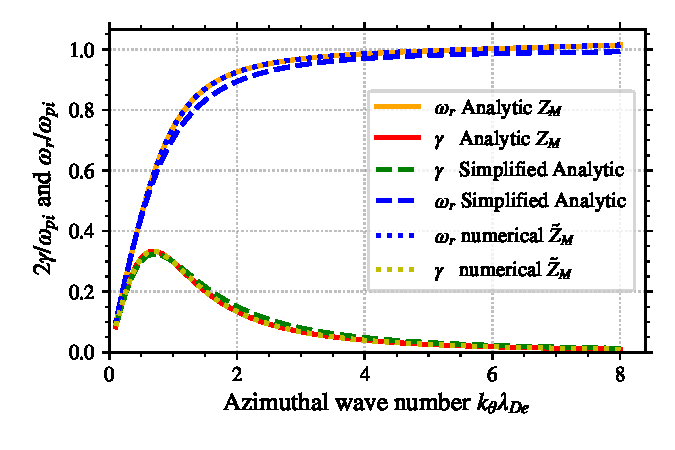
\includegraphics[width=0.7\textwidth]{IAW_Maxw}
    \caption{IAW frequency $\omega_r$ and growth rate $\gamma$ (scaled by a factor of two) for a Maxwellian distribution function using the Freid and Conte function (labelled Analytic $Z_M$), the numerical estimation of $\tilde{Z}_M$, and the simplified analytic expressions of \cref{eq-MIAW}. }
    \label{fig-IAW_Maxw}
  \end{figure}
  
  We can see that the three approaches give almost the same solutions.
  The growth rates are all overlapping, hence it is difficult to see the differences.
  For $\omega_r$, the simplified analytic expression returns a slightly different result, but the difference is negligible.
  The numerical evaluation of $\tilde{Z}_M$ gives the same result as the analytic evaluation.
  
  \Cref{fig-IAW_druv} shows the effect of a Druyvesteyn electron distribution compared to a Maxwellian.
  We recall that a Druyvesteyn distribution follows the expression
  \begin{equation} \label{eq-druyv}
    f_{D}(v) = v_{th}^{-1} C2 \exp \lp -C1 \frac{\norm{v}^4}{v_{th}^4}  \rp ,
  \end{equation}
  
  where $C1 \simeq \Gamma(3/4)^2 \Gamma(5/4)^{-2}/4 \simeq 0.457 $ and $C2 =\Gamma(3/4)^{1/2} \Gamma(5/4)^{-3/2}2^{-3/2}  \simeq 0.453$ are two normalizing constants, so that the density and the thermal velocity $v_{th}$ are consistent with the Maxwellian distribution.
  The electron density used is $n_e=\sn{1}{17}\,\meter^{-3}$ and the electron temperature is $\Te=50\,\volt$, the ion temperature is $\Ti=0.1\,\volt$, and the drift velocity is $u_e=\sn{1.8}{6}\,\meter\per\second \simeq 300 c_s$ with $c_s=\lde \opi\simeq 6\,\kilo\meter\per\second$.
  We see in \cref{fig-IAW_druv} that the impact of the Druyvesteyn \ac{EVDF} on the \ac{IAW} dispersion relation is small, except that the maximum growth rate is decreased by $15\%$.
  
  \begin{figure}[!hbt]
    \centering
    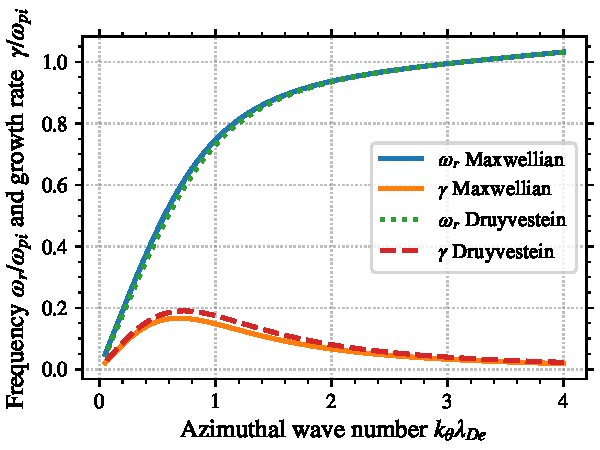
\includegraphics[width=\defaultwidth]{IAW_druv}
    \caption{IAW frequency and growth rate for a Maxwellian distribution function using the Freid and Conte function and a Druyvesteyn distribution evaluated with the numerical estimation of $\tilde{Z}$. }
    \label{fig-IAW_druv}
  \end{figure}
  \Cref{fig-valition-solver} shows the evolution of the most growing wave with the electron drift velocity for both the Maxwellian and the Druyvesteyn \ac{EVDF}.
  An illustration of the two distribution functions with a drift equal to the thermal velocity can be seen in \cref{fig-valition-solver}.{\bf b}.
  We see that, as obtained in the analytic dispersion relation \cref{eq-MIAW}, the growth rate is proportional to the drift velocity when $u_e \ll v_{th}$.
  In addition, the wave corresponding to the maximum growth rate depends only weakly of the drift velocity, and we find a good agreement with the analytic values $k_{\theta} \lde =1/\sqrt{2} \simeq 0.707$ and $\omega / \opi = 1/\sqrt{3} \simeq 0.577$. 
  Lastly, the shape of the \ac{EVDF} seems to affect only weakly the result.
  
  \begin{figure}[!hbt]
    \centering
    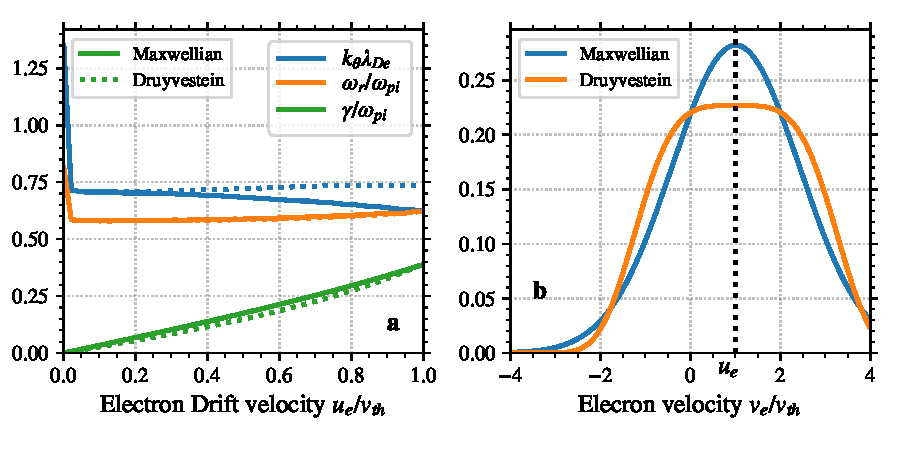
\includegraphics[width=0.8\textwidth]{comp_Maxw_Druyv_IAW.pdf}
    \caption{({\bf a}) Evolution as a function of the electron drift velocity $u_e$ of the maximum growth rate $\gamma$ and the corresponding wavenumber $k_{\theta}$ and frequency $\omega$ of the \acs{IAW} for both a Maxwellian and a Druyvesteyn \acs{EVDF}, supposing the ions Maxwellian;({\bf b}) the two distribution function for $u_e/c_s = 300$.}
    \label{fig-valition-solver}
  \end{figure}
  
  \FloatBarrier
  
  \paragraph{Electron Cyclotron Drift instability\\}
    

  
  \Cref{fig-ECDI_druv} shows the frequency and the grow rate for the \ac{ECDI}, defined by \cref{eq-drECDI}, in the same conditions that the \ac{IAW} results, with $k_r \lambda_{De} = 0.05 $.
  The infinite sum over the cyclotron resonances is stopped at $N_{max} = 20$.
  We see in \cref{fig-ECDI_druv} that the cyclotron resonances are present for both distribution functions, and the wave frequency and the growth rate are not much affected by the shape of the \ac{EVDF}.
  For very small radial wavenumber, the numerical resolution crashes, as the argument in $Z(\eta)$ diverges.
  However, in the limit $\eta \rightarrow \infty, Z(\eta) \rightarrow  \frac{1}{\eta}$.
  Hence, we still obtain the cyclotron resonances, as shown in \citet[Fig. 2]{janhunen2018}.
  
  \begin{figure}[!hbt]
    \centering
    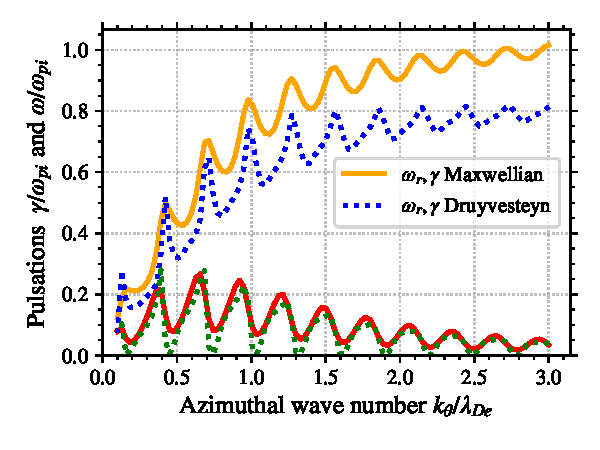
\includegraphics[width=\defaultwidth]{ECDI_druv}
    \caption{\acs{ECDI} frequency and growth rate for a Maxwellian distribution function using the Freid and Conte function and a Druyvesteyn distribution evaluated with the numerical estimation of $\tilde{Z}$, the radial wave number is $k_r \lambda_{De} = 0.05$. The \acs{IAW} \acs{DR} using Maxwellian VDFs is shown }
    \label{fig-ECDI_druv}
  \end{figure}

  We also see in \cref{fig-ECDI_druv} that the \ac{ECDI} \ac{DR} presents the resonances around the \ac{IAW} \ac{DR}.
  This is why in case of resonance broadening, the \ac{ECDI} converged toward a \ac{IAW}-like dispersion relation.

\let\rightmark=\oldrightmark
